\chapter{delete}

\section*{Lösung}

Nach dem Löschen eines Knotens in einem Suchbaum soll der durch die Löschoperation entstehende Baum wieder ein Suchbaum sein, und die in Abschnitt~\ref{ch:binarytree} aufgeführten Kriterien erfüllen.

Die Ausführung der Löschoperation findet sich im Skript (Teil 2) auf Seite 147 ff., aus der sich die korrekte Antwort herleiten lässt.
\\

Etwas ausführlicher beschreiben \textit{Ottmann und Widmayer} die Knoten, die an die Stelle des gelöschten Knotens treten können, als den \textit{symmetrischen Vorgänger} bzw. den \textit{symmetrischen Nachfolger} (vgl.~\cite[288 f.]{OW17e})\footnote{
in Abschnitt 5.1.2, ebenda, wird die \textit{Inorder}-Durchlaufordnung auch als \textit{Symmetrische Reihenfolge} bezeichnet.
}.
\\

Der \textbf{symmetrischen Vorgänger} \textit{u} des Knotens \textit{p} ist der Knoten im \underline{linken Teilbaum} von \textit{p}, der am weitesten \underline{rechts} steht.
\\

Der \textbf{symmetrischen Nachfolger} \textit{v} des Knotens \textit{p} ist der Knoten im \underline{rechten Teilbaum} von \textit{p}, der am weitesten \underline{links} steht\footnote{
    Da wir einen Suchbaum vorliegen haben, gilt als Voraussetzung für den \textit{symmetrischen Nachfolger}, dass der Schlüssel \textit{z} des Knotens \textit{v} größer als der Schlüssel \textit{x} des Knotens \textit{p} ist, und für den \textit{symmetrischen Vorgänger}, dass der Schlüssel \textit{y} des Knotens \textit{u}  kleiner als der Schlüssel \textit{x} des Knotens \textit{p} ist
}.
\\

Die folgende Darstellung verdeutlicht den Zusammenhang von einem Knoten mit seinem symmetrischen Vorgänger {bzw.} Nachfolger.
In dem  {geg.} Suchbaum gilt, dass der Betrag der Differenz von $x - y$ bzw. $x - z$ jeweils der kleinste Betrag aller möglichen Beträge ist, die aus der Menge der möglichen Schlüssel des linken {bzw.} rechten Teilbaums mit $x$ gebildet werden können.
Die beiden Knoten nähern sich mit ihrem Schlüsselwert also dem Schlüsselwert des Knotens \textit{p} am ehesten an.


\begin{figure}[h]
    \centering
    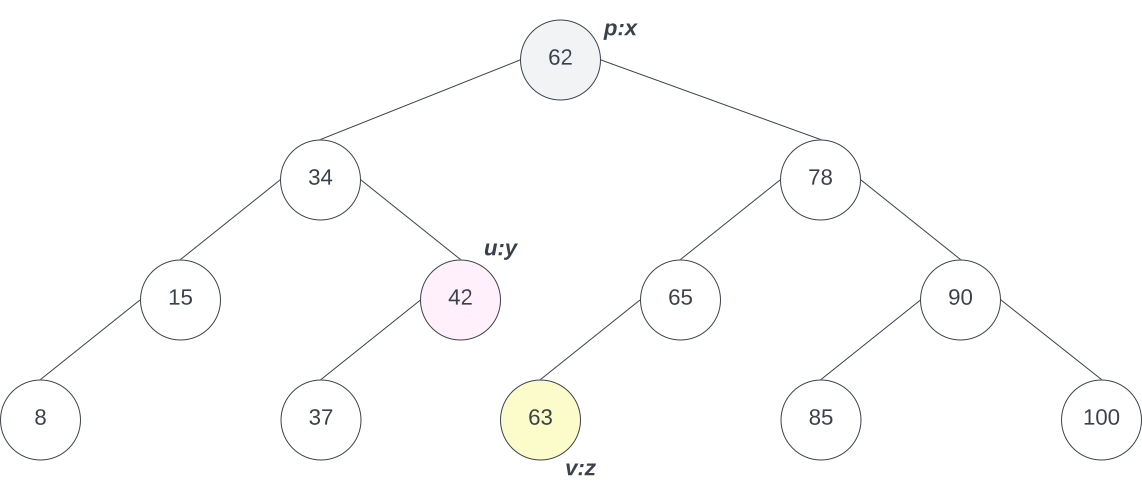
\includegraphics[
        width=16cm,
        keepaspectratio,
    ]{chapters/3. delete/img/symm}
    \caption{Der symmetrische Vorgänger \textit{u} und der symmetrische Nachfolger \textit{v} des Knotens \textit{p}.}

\end{figure}


Mit dem Wissen kann man den Knoten \textit{p} durch den Knoten \textit{u} oder den Knoten \textit{v} ersetzen.
Aufgrund der Tatsache, dass die gelöschten Knoten die Eigenschaft \textit{symmetrischer Vorgänger} bzw \textit{symmetrischer Nachfolger} besitzen, können die Knoten keinen {bzw.} einen linken oder rechten Nachfolger in Form eines Blattes bzw. inneren Knotens
haben, weshalb sich das Ersetzen dieser weggefallenen Knoten als trivial erweist\footnote{
Hinweise hierzu im Skript (Teil 2) auf Seite 149 und in~\cite[269]{OW17e}: ``Der Knoten \textit{q} [\textit{v}] ist der am weitesten links stehende innere Knoten im rechten Teilbaum von \textit{p} und kann daher höchstens einen inneren Knoten als rechten
    Sohn haben.``
}

\begin{figure}[h]
    \centering
    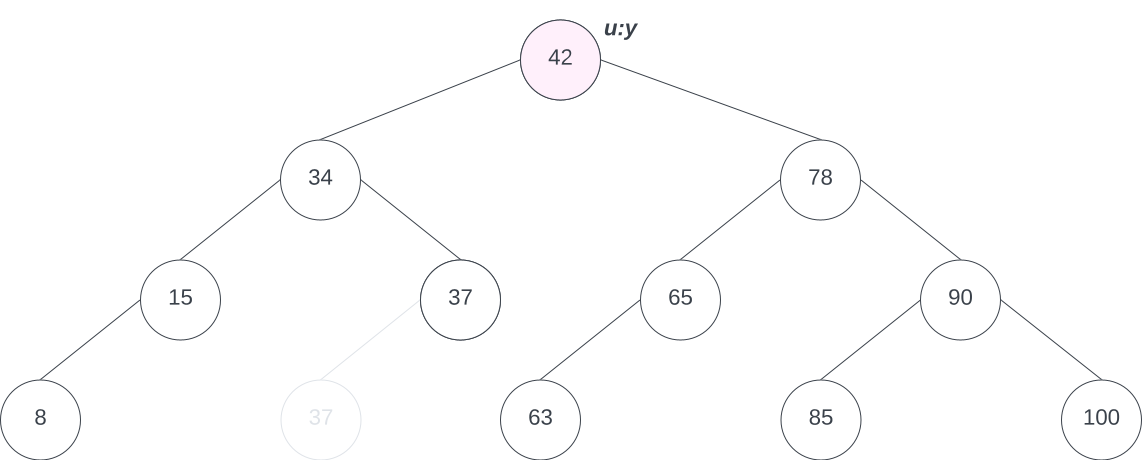
\includegraphics[
        width=16cm,
        keepaspectratio,
    ]{chapters/3. delete/img/symm_42}
    \caption{Löschen des Knotens \textit{p} und Ersetzen durch seinen symmetrische Vorgänger \textit{u}.}

\end{figure}

\begin{figure}[h]
    \centering
    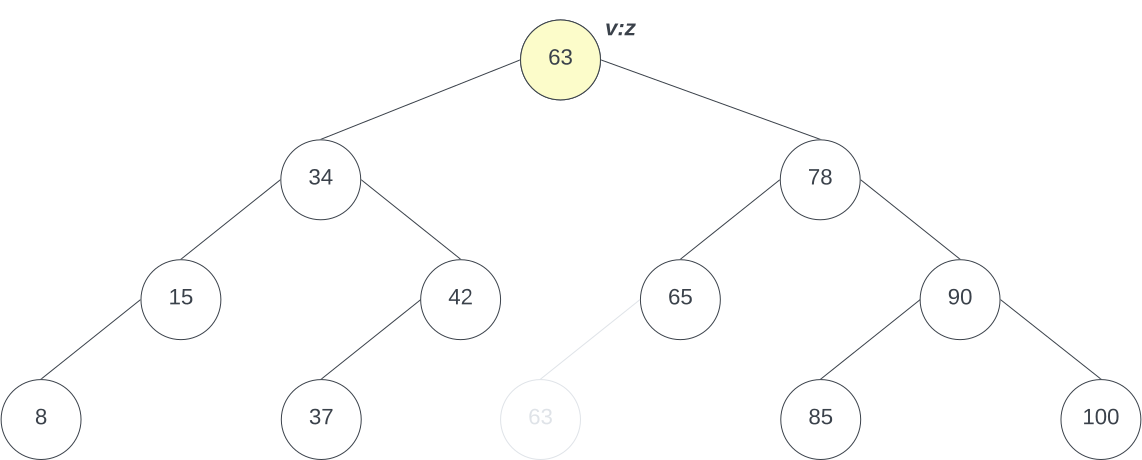
\includegraphics[
        width=16cm,
        keepaspectratio,
    ]{chapters/3. delete/img/symm_63}
    \caption{Löschen des Knotens \textit{p} und Ersetzen durch seinen symmetrische Nachfolger \textit{v}.}

\end{figure}
